% 编译：tectonic -X compile --outdir <输出目录> main.tex（或 xelatex main.tex）
% 版式：表头 + 右上角照片、章节横线、加粗引导词 bullet、右侧日期
% 内容依据：本地 personal-web 项目（_data/cv.yml、socials.yml、papers.bib）、
%           Hushfusion_Forge/README.md、fusion-sim/README.zh-CN.md 及公开主页 logos-42.github.io
% 说明：同目录下的第三方简历 PDF 仅为版式参考，不作为任何内容来源，也不随站点发布。
\documentclass[10pt,a4paper]{article}

% ---------- 基础包 ----------
% fontset=fandol 使用 TeX Live 自带的 Fandol 中文字体，不依赖 macOS 系统字体名
% 若本机确认装有「Songti SC / PingFang SC」且想用系统字体，可改为 fontset=macnew
\usepackage[fontset=fandol]{ctex}
\usepackage{geometry}
\usepackage{titlesec}
\usepackage{hyperref}
\usepackage{fancyhdr}
\usepackage{enumitem}
\usepackage{xcolor}
\usepackage{graphicx}

% ---------- 页面设置 ----------
\geometry{left=1.6cm, right=1.6cm, top=1.3cm, bottom=1.3cm}
\pagestyle{fancy}
\fancyhf{}
\renewcommand{\headrulewidth}{0pt}
\cfoot{\small\thepage}

\definecolor{linkblue}{RGB}{30,80,150}
\hypersetup{colorlinks=true, urlcolor=linkblue, linkcolor=linkblue, citecolor=linkblue, pdfborder={0 0 0},
  pdftitle={刘元杰 · 简历 / CV}, pdfauthor={刘元杰 (Yuanjie Liu)},
  pdfsubject={磁约束聚变理论模拟与 AI 科研系统}}

% ---------- 标题样式 ----------
\titleformat{\section}{\large\bfseries\raggedright}{}{0em}{}[\titlerule]
\titlespacing*{\section}{0pt}{7pt}{3pt}

% ---------- 自定义命令 ----------
\newcommand{\resumeItem}[1]{\item \small #1}
\newcommand{\resumeSubheading}[4]{
  \item
  \begin{tabular*}{0.97\textwidth}{l@{\extracolsep{\fill}}r}
    \textbf{#1} & #2 \\
    \textit{\small #3} & \textit{\small #4} \\
  \end{tabular*}
}

% --------------------------------
\begin{document}

% ---------- 表头 ----------
% 照片用 LaTeX 内核 picture 环境定位到右上角：单遍编译即可显示，不依赖 TikZ remember picture
% 找不到 portrait.jpg 时在 PDF 里给出可见提示，避免静默跳过难以排查
\noindent
\IfFileExists{portrait.jpg}{%
\begin{picture}(0,0)
  \put(442,-84){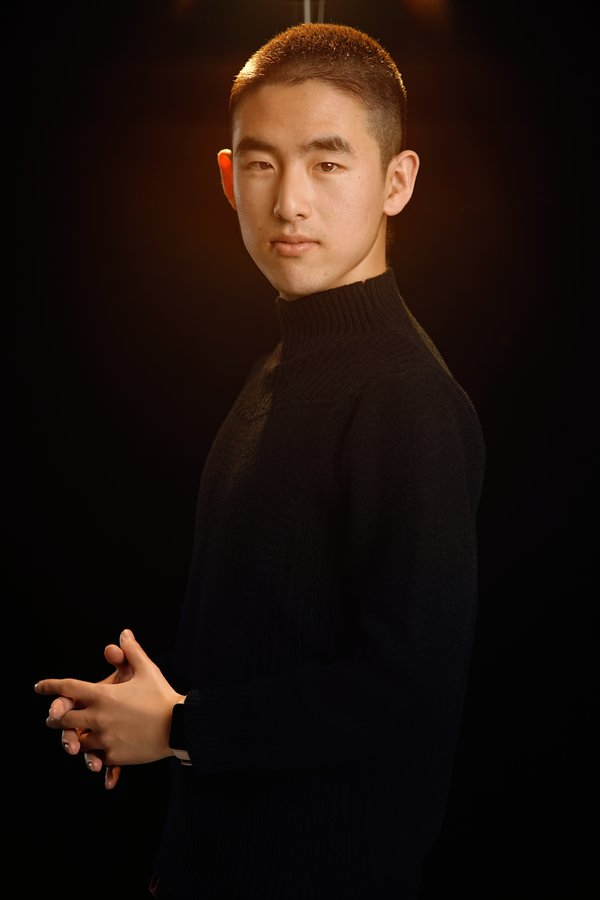
\includegraphics[width=2.2cm]{portrait.jpg}}
\end{picture}%
}{%
\begin{picture}(0,0)
  \put(400,-24){\textcolor{red}{\small 缺图：portrait.jpg}}
\end{picture}%
\typeout{^^J WARNING: portrait.jpg not found - photo skipped.^^J}%
}

\begin{center}
\begin{minipage}{0.70\textwidth}\centering
  {\Huge\bfseries 刘元杰}\\[5pt]
  {\small \href{mailto:2844169590@qq.com}{2844169590@qq.com} $\cdot$ 13115718038 $\cdot$ 微信 vuca335507 $\cdot$ 现居杭州}\\[2pt]
  {\small \href{https://logos-42.github.io/}{个人主页} $\cdot$ \href{https://github.com/logos-42}{GitHub} $\cdot$ \href{https://orcid.org/0009-0007-4845-641X}{ORCID} $\cdot$ \href{https://arxiv.org/abs/2511.11619}{arXiv} $\cdot$ 随时到岗}\\[5pt]
  {\bfseries 求职意向：等离子体理论模拟研究员 $|$ 等离子体加热与诊断系统研究员/工程师}
\end{minipage}
\end{center}
\vspace*{0.5cm}

% ---------- 教育背景 ----------
\section{教育背景}

\noindent\textbf{天津商业大学 · 自动化信息工程学院}\hfill\textbf{2020.09 -- 2024.06}\\
\textit{\small 自动化与人工智能方向 · 工学学士}

\begin{itemize}[leftmargin=0.15in, topsep=2pt]
\resumeItem{相关课程：线性代数、概率统计、数理逻辑、系统架构；以自学方式补充理论物理与磁约束聚变基础。}
\end{itemize}

% ---------- 研究概况 ----------
\section{研究概况}

\begin{itemize}[leftmargin=0.15in, topsep=2pt]
\resumeItem{独立研究者，围绕磁约束聚变开展工程化研究：以 Go 实现 HUSHFUSION Forge 电磁线圈设计闭环（磁镜位形的真空静磁学建模、等预算自动搜索、独立 Python 复核），以 Python / JAX 搭建 fusion-sim 聚变数字仿真工作台（TORAX / Gym-TORAX 输运仿真与 gym-$\mu$-FRC 控制环境）；并以第一作者撰写 arXiv 预印本（DIAP）。}
\resumeItem{面向磁镜--仿星器耦合位形的理论模拟与诊断数据链路，能力集中在磁场位形建模与优化、输运与控制仿真、数值实验门禁与可复现验证、工程化实现（Go / Python / JAX），以及预印本与技术文档写作。}
\end{itemize}

% ---------- 聚变研究项目 ----------
\section{聚变研究项目}

\begin{itemize}[leftmargin=0.15in, label={}, topsep=2pt]

\item \textbf{HUSHFUSION Forge · 电磁线圈设计闭环}\hfill\textit{\small Go, Python（独立复核）, 磁镜位形}
\begin{itemize}[topsep=1pt, label=\textbullet]
\resumeItem{\textbf{问题：}聚变装置线圈设计依赖手工迭代，单次实验只产出一个设计，设计知识无法被后续复用。}
\resumeItem{\textbf{方法：}构建「参数化设计 $\to$ 磁场物理 $\to$ 目标函数 $\to$ 搜索 $\to$ 设计注册表 $\to$ 设计规则」闭环；磁场用圆环电流闭式解（完全椭圆积分 AGM）与独立分段 Biot--Savart 交叉验证；目标函数含场强、镜比、可用场体积、纹波、造价与约束罚；人工基线为 Helmholtz 中央室 + 镜喉（中场平均场 1.0 T）。}
\resumeItem{\textbf{验证：}以等预算对照实验比较多种搜索策略，机器设计在多个随机种子下稳定优于人工基线；通过自动化验收门与跨语言 oracle 交叉校验保证结果可复现。}
\end{itemize}

\item \textbf{fusion-sim · 聚变数字仿真工作台}\hfill\textit{\small Python, JAX, TORAX, Gymnasium}
\begin{itemize}[topsep=1pt, label=\textbullet]
\resumeItem{\textbf{问题：}验证现有 AI 仿真栈的本机可运行性，并判断自研物理模型能否做成可训练、可验证的控制问题。}
\resumeItem{\textbf{方法：}A 线跑通 TORAX（可微 1-D 输运）+ Gym-TORAX（Gymnasium 控制环境）+ ITER ramp-up；B 线实现 gym-$\mu$-FRC v0（$\mu$ 动力学 TD1--TD21、FRC 窗口 FC11b/FC5b、RMF 代价、RL 环境）；与 Lean 4 形式化逐条对齐、$\mu\to 0$ 极限回归、多 seed 与穷举参考解对照。}
\resumeItem{\textbf{验证：}以自动化门禁覆盖多 seed 训练、对照组与穷举参考解，并用缺陷注入确认门禁能捕捉实现错误；依赖版本固定以保证可复现。}
\end{itemize}

\end{itemize}

% ---------- 理论物理与形式化 ----------
\section{理论物理与形式化验证}

\begin{itemize}[leftmargin=0.15in, topsep=2pt]
\resumeItem{\textbf{理论物理：}以自学方式补充理论物理基础，围绕数学物理与形式化方法开展独立研究，形成 6 篇独立作者预印本（2026）。}
\resumeItem{\textbf{Lean 4 形式化：}以 Lean 4 / Mathlib 把定理写成机器可验证证明，涵盖 \href{https://github.com/logos-42/NODS}{NODS}（新数学对象发现系统）、\href{https://github.com/logos-42/Hibs-Physics}{Hibs-Physics}、\href{https://github.com/logos-42/YangMillsPhysics}{YangMillsPhysics}，零 sorry、零 warning。}
\end{itemize}

% ---------- AI 科研与智能体系统 ----------
\newpage
\section{AI 科研与智能体系统}

\begin{itemize}[leftmargin=0.15in, label={}, topsep=2pt]
\item \textbf{AI 科研工作流与智能体系统}\hfill\textit{\small Go, Rust, TypeScript, Python}
\begin{itemize}[topsep=1pt, label=\textbullet]
\resumeItem{具备 AI 科研工作流编排、多智能体系统设计与 AI 操作系统相关能力；以 Go 实现已可运行的全自动多智能体工作流软件，覆盖工作流编排与任务自动执行。}
\resumeItem{开源项目：DIAP 去中心化智能体身份协议（零知识证明 + 混合 P2P）、bolloon 智能体资源交流网络、Hib-OS、headless。}
\resumeItem{其他工程实现：仿真数据自动化评估工具（Python / AutoGen，指标体系与仿真数据处理）、多设备参数同步与算力调度框架（Rust / Python）、复数域高维表示验证模型（PyTorch）。}
\end{itemize}
\end{itemize}

% ---------- 经历 ----------
\section{研究与实践经历}

\begin{itemize}[leftmargin=0.15in, label={}, topsep=2pt]

\resumeSubheading{浙大滨江研究院 · 人工智能与系统研究方向}{2025.08 -- 2026.05}{研究助理 / 研究工程师}{}
\begin{itemize}[topsep=1pt, label=\textbullet]
\resumeItem{参与多智能体系统与分布式计算课题研究，负责协议机制建模与仿真实验。}
\resumeItem{完成大模型及智能体性能评估，设计评估流程与对比实验。}
\resumeItem{协助撰写研究报告与技术文档。}
\end{itemize}

\resumeSubheading{GAP · 独立研究与技术探索}{2024.07 -- 2025.08}{}{}
\begin{itemize}[topsep=1pt, label=\textbullet]
\resumeItem{独立开展 AI 智能体与分布式系统技术探索，负责产品规划、系统架构设计与核心代码实现。}
\resumeItem{设计并实现多智能体协作原型与算力调度系统。}
\end{itemize}

\end{itemize}

% ---------- 论文与成果 ----------
\section{论文与成果}

\begin{itemize}[leftmargin=0.15in, topsep=2pt]
\resumeItem{\textbf{第一作者 · arXiv 预印本 (2025)：}Yuanjie Liu, Wenpeng Xing, Ye Zhou, Gaowei Chang, Changting Lin, Meng Han. \emph{DIAP: A Decentralized Agent Identity Protocol with Zero-Knowledge Proofs and a Hybrid P2P Stack}. \href{https://arxiv.org/abs/2511.11619}{arXiv:2511.11619}；署名单位：浙大滨江研究院。}
\resumeItem{\textbf{独立作者预印本 6 篇 (2026)：}含 \emph{Counting, Not Confinement: The Yang--Mills Conjecture in the Flowing-Space Gauge Theory}、\emph{The Sink Is a Flattening} 等；完整列表见 \href{https://logos-42.github.io/publications/}{个人主页 Publications}。}
\resumeItem{\textbf{开源项目：}\href{https://github.com/logos-42/hushfusion-forge}{hushfusion-forge}（Go）、\href{https://github.com/logos-42/fusion-sim}{fusion-sim}（Python）、\href{https://github.com/logos-42/NODS}{NODS}、\href{https://github.com/logos-42/bolloon}{bolloon}（4 stars / 3 forks）等；详见 \href{https://github.com/logos-42}{GitHub}。}
\end{itemize}

% ---------- 能力 ----------
\section{研究与技术能力}

\begin{description}[leftmargin=2.2cm, labelsep=0.3cm, topsep=2pt, itemsep=1pt]
\item[聚变与仿真] 磁镜线圈位形设计与优化、真空静磁场计算（椭圆积分 / Biot--Savart）、TORAX 1-D 输运仿真、Gym-TORAX / gym-$\mu$-FRC 控制环境、FRC 窗口与 RMF 代价；等预算搜索与设计注册表
\item[数值与语言] Go, Python, Rust；JAX / Gymnasium；数值实验设计、等预算 benchmark、门禁与跨语言 oracle 交叉验证、可复现实验报告
\item[数学与形式化] 线性代数、概率统计、数理逻辑；理论物理（自学）；Lean 4 / Mathlib 形式化证明（零 sorry）
\item[AI 科研系统] AI 科研工作流、智能体工作流编排、多智能体系统、AI 操作系统；多智能体协议（DIAP / bolloon）
\item[系统与协作] 分布式系统、多设备参数同步、系统架构设计；英文文献阅读、研究报告与预印本撰写
\end{description}

\end{document}
